\documentclass{article}
\usepackage[margin=1.25in]{geometry}
\usepackage{fancyhdr}
\usepackage{graphicx}
\usepackage{vhistory}
\usepackage[parfill]{parskip}
\graphicspath{{../Images/}}

\renewcommand{\baselinestretch}{1.5}

% Set fancy looking header/footer and move page number to the right
\pagestyle{fancy}
\fancyhead{}
\fancyfoot{}
\fancyfoot[R]{\thepage}

\patchcmd{\section}{-3.5ex \@plus -1ex \@minus -.2ex}{-3.5ex \@plus -1ex \@minus -.2ex\setlength{\leftskip}{0cm}}{}{}
\patchcmd{\subsection}{-3.25ex\@plus -1ex \@minus -.2ex}{3.25ex\@plus -1ex \@minus -.2ex\setlength{\leftskip}{1cm}}{}{}
\patchcmd{\subsubsection}{1.5ex \@plus .2ex}{1.5ex \@plus .2ex\setlength{\leftskip}{2cm}}{}{}

\begin{document}
    \pagenumbering{gobble}
    \begin{titlepage}
    \begin{center}
        \vspace*{1cm}

        \Huge
        \textbf{User's Guide for Cloud Backup}

        \vspace{.5cm}
        \LARGE
        Captain CyBeard: Neil Before Us

        \vspace{1cm}

        \textbf{Ryan Breitenfeldt \textbar\ Noah Farris\\ Trevor Surface \textbar\ Kyle Thomas}

        \vspace{.2cm}
        \Large
        May 4, 2020

        \vspace{2cm}
        
\includegraphics[scale=1]{logo}

        \vfill

        Washington State University Tri-Cities\\
        CptS 423 Software Design Project 2

    \end{center}
\end{titlepage}




    \tableofcontents
    \newpage
    \listoffigures


    \newpage
    \begin{versionhistory}
        \vhEntry{2.1}{12.04.2019}{TS}{Provided more grammatical checking along with a Reference Recomendation}
        \vhEntry{2.0}{12.04.2019}{KT}{Added priority section \& final edits}
        \vhEntry{1.2}{12.03.2019}{KT}{Grammar edits and wording}
        \vhEntry{1.1}{11.16.2019}{NF}{Grammar edits and wording}
        \vhEntry{1.0}{11.15.2019}{RB NF TS KT}{First Final Doc}
        \vhEntry{0.9}{11.14.2019}{KT}{Spelling \& grammar edits}
        \vhEntry{0.8}{11.12.2019}{TS}{Added more components to subsections for length}
        \vhEntry{0.7}{10.29.2019}{NF}{Edits to whole doc}
        \vhEntry{0.6}{10.29.2019}{KT}{Edits}
        \vhEntry{0.5}{10.28.2019}{NF}{Background}
        \vhEntry{0.4}{10.28.2019}{RB}{Introduction}
        \vhEntry{0.3}{10.15.2019}{TS}{Completed Overview}
        \vhEntry{0.2}{10.10.2019}{RB NF TS KT}{Filled in Environment \& Operation sections}
        \vhEntry{0.1}{09.27.2019}{KT}{Document Creation}
    \end{versionhistory}
    \newpage


    \pagenumbering{arabic}
    \section{Introduction}
    This requirements specification document will go over the requirements for the Virtual Machine file Downloader for Cypherpath's Resiliency Platform that was outlined in the
    \texttt{Project Plan} \cite{projectplan}.
    The document will cover how the application will provide a solution for users to easily upload their Virtual Machine files to the Resiliency Platform.
    Providing details on how the users will interact with the application through a web interface. This document will be understood and agreed
    upon by both the customer (Cypherpath) and the software development team (Captain CyBeard).

    Subsequent sections will include, background information on Cypherpath and their Resiliency Platform. An overview of the application, what it
    will Accomplish. The environment the application will execute in. How users will interact the application. Additionally includes the priority of the cloud platforms that the application will support.

	The Cypherpath Resiliency Platform tool is a product that provides their customers the ability to upload virtual machines, network configurations and more, into 
    self-contained digital environments. This enables their customers to quickly recover from attacks such as ransomware. Right now, customers have to manually download their virtual disk images from
    the various cloud platforms they are hosted on, and then upload those to the Resiliency Platform. Cypherpath has requested a web application that will enable users to have their virtual disk images go
    directly from the cloud platform into the Resiliency Platform, cutting out the multi-step process of downloading and then uploading large virtual disk images.
	
    \section{Background}
    Cypherpath's Resiliency Platform started out as a platform where the U.S. Military could emulate the networks of countries and simulate cyber attacks between the countries in order to
    learn about the strength and weaknesses of the countries simulated. After proving its usefulness in this market, Cypherpath entered the commercial market and provides it platform as a service to
    companies and local governments alike to provide resiliency to these entity's network infrastructures. Resiliency in the cyber sense means that systems and networks are secure, recoverable and
    continuous. Customers of Cypherpath enjoy a readiness of their technological resources, and can rapidly adjust and adapt those resources when failures, damages or attacks occur in order to keep their business running smoothly.

    This project will become a component of the Resiliency Platform by enabling Cypherpath's customers to more easily migrate their virtual assets into the platform. Currently customers have to download
    their virtual assets onto their local machine and then upload them into the Resiliency Platform. This project will simplify this process by having the Resiliency Platform download the virtual asset directly
    into its infrastructure. The software development team will not be integrating the application with the Resiliency Platform. The product delivered to Cypherpath will be a standalone web application that downloads
    digital assets from various cloud platforms. Upon completion of the project, Cypherpath will integrate the web application into their Resiliency Platform.

	%This project will give Cypherpath users a simple means of directly transferring virtual disk images from various cloud platforms directly into
    %Cypherpath's Resiliency Platform, providing more value to the customer in the process.

	
    \section{Overview}
    The purpose of this application is to allow users to download virtual disk images from online cloud platforms, to local file storage.
    The application itself will operate as a web server using Python3 and Django2. Users will start the application by navigating to the URL pointing to the application.
    Once at the main page the user will
    provide a URL to their account on an external cloud platform. Once the application processes the URL to determine which cloud platform the URL points to, the user is
    then asked to provide their credentials to authenticate
    to that platform. After authentication, the application will use the API of the cloud platform and show the user their Virtual Disk Image (vdi) for that machine.
    The User will be able to navigate their directory structure and select which files and folders to download locally to their desktop.
    When the user clicks the download button the application will use another API call to download the files onto their PC.

    The application will be written with Python3 and Django2, including the requests libraries for API calls, Authentication libraries like SAML
    and standard libraries. To install the application, Cypherpath will integrate the Django web application into their environment along with installing (if not installed already)
    the libraries for interacting with the external cloud platforms and authentication API's. Users of the application will not need to install any software since most operating systems come
    with a web browser which will interact with the application on the user's end.

    %The application only allows users to view the files from VM's they own, and download those file locally to the machine they 
    %are running the application through. The users will have the ability to provide either a VMware URL to download from, or an
    %Amazon Web Services (AWS) VM URL. The application will be designed with modularity to allow further development with different 
	%VM service providers such as Citrix, Google Drive and DropBox. If time allows, these will be developed incrementally, with 
	%Citrix being the next highest priority and then Google Drive and DropBox.

	%\large ?? WHAT IS THE WEBHOST INFORMATION ?? 
	%?? Also, I'm not sure that understand Trevors notes on this ??
	
    \section{Environment}
	%\large This application will preside in Cyperpath's suite of applications and will connect to cloud services through API calls. 
    %!! NEED MORE INFO FROM CYPHERPATH HERE !!
    The next sections will go over the environment the application will reside in. This will include the web application, authentication API's, cloud storage API's and the local storage
    of the machine running the application. During development this will be the users machine, but Cypherpath will be using their storage scheme for production.
	
    \begin{figure}[h]
    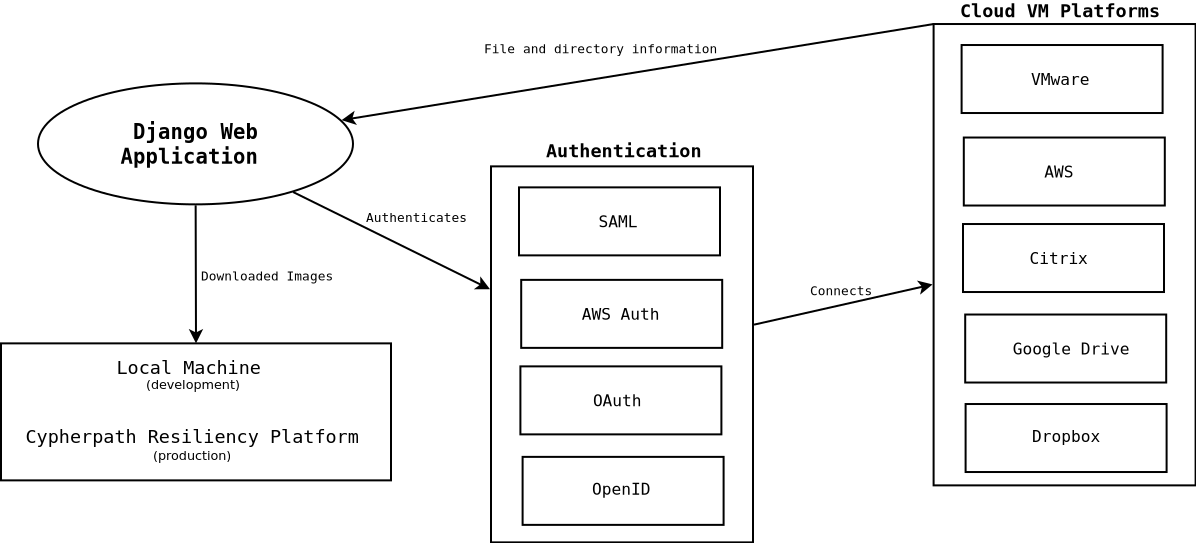
\includegraphics[scale=.4]{downloader_env}
        \caption{A visual representation of the applications environment.}
    \end{figure}


        \subsection{Web Application}
        The web server for the application during development will be Django's built in development server and when the project is completed, Cypherpath will integrate
        the web application into their existing ecosystem using their webserver. The Django application will host the functionality of the application, including HTML templates for the 
        web pages, where users provide Virtual Machine URLs and browse their directories. Additionally, the Django framework will allow the usage of python classes that will enable the 
        back-end operation of the application.

        
        \subsection{Authentication API's}
        The application will authenticate to the cloud platforms with various authentication methods and API's. The application will support
        SAML, AWS Authentication, OpenID and OAuth. The application will be designed in a modular fashion so that more authentication methods can be easily added later.
        The authentication will provide a token to verify the users for their cloud platform, the application will not provide previous states for the use of the 
        website, nor will it save previous URL's entered. The token will be passed to the request for access to the URL provided.


        \subsection{Cloud Storage API's}
        Once the application is authenticated to a cloud storage platform it will gather the directory structure for showing to the user and allowing them to select
        which of their files they would like to download. The application will support interacting with VMware, Amazon Web Services, Citrix, Google Drive and Dropbox. The API's
        that are necessary for the communication, will request the directory structure of their cloud storage and provide it to the user so they can select which virtual disk
        images they would like to download. Like the authentication modules, the modules
        for interacting with the cloud API's will need to be designed so that adding support for other cloud platforms will be possible.


        \subsection{Local Storage}
        Once the user has selected which files to download from their cloud platform, the application will download those
        files to the user's local storage. The application will download all of the user's selected files from the cloud platform to their local storage.
        The local storage location will be determined by the web browser, the application will serve the files from the cloud platform to the user's web browser. Nothing else 
        needs to be done with the files because after the application is finished and Cypherpath has integrated the web application into 
        their platform, they will direct the downloads where they need them.


    \section{Operation}
    In the following sections the operation of the application will be described, including starting the application
    (invocation) from the user's perspective and the web server administrator, the commands the application uses and finally, how users and administrators will terminate the application.

        \subsection{Invocation}
        During development the application will be started using Django's built-in webserver and
        the user will not need to be authenticated to use the application. To invoke the application the user will simply enter the URL for the application (such as http://localhost:8080).
        They will then be presented with the main screen of the application. The screen will have a single input text box for a user to insert a URL. Additionally 
        a submit button will be provided for them to continue to step through the application. 

        To start the development server, the developer/mock web administrator will use the following command in the Django project directory containing the \textit{manage.py} file.
        \begin{verbatim}
        $ python manage.py runserver
        \end{verbatim}

        The user will now be able to use their web browser to visit the main page.

        The user interface and invocation of the application are simple. Later when Cypherpath integrates the application into their Resiliency Platform, invocation by the user will be from within Cypherpath's
        platform. Cypherpath does not have preferences on the user interface since they will be adding their own style, layout, themes, etc.\ to the user interface. The server side of the application will be invoked
        from Cypherpath's web server that serves their platform.

        %%If there is an error in the initial URL provided the user will be prompted with an error that either the machine doesn't exist or cannot be reached, or if invalid credentials 
        %%were provided, will be prompted as such. %% Shouldn't this be in the "Enter URL" section?

        \subsection{User Actions}
        This section covers how the user will interact with the application and how entering the application, displaying the file structure, downloading virtual disk images and error catching 
        will be implemented.

            \subsubsection{Enter URL}
            On the main page of the application the user will be presented with a textbox where they will enter a URL that goes to their cloud platform. The text box will be centrally located with a design to
            help users clearly see where to input the URL. The box will also have shadow text requesting input. Once a URL is entered and submitted the application will figure out which cloud platform the URL
            belongs to, through a GET request to the URL. If an error occurs with the GET request the user will be notified of the error. If the request is successful then the user will be prompted to
            provide their login credentials to their cloud platform, on a pop-up window. The authentication will be verified with the platform they are using, (for example: SAML for VMware or AWS Auth for AWS).
            Once authenticated the application will present the user with their files and folders that are on that platform.
            
            \subsubsection{Display File Structure and Download Selected Files}
            Once the user has selected a cloud platform and is authenticated, they will be presented with their directory structure on that platform. They will only see high level directories initially,
            however, they will be able to open the directories to see files located within. They can use this information to verify all files were retrieved from the cloud once downloaded and select which
            files to download. After selecting the files and folders the user wants, they will click the download button, which initiates the download of their selected files from the cloud platform.
            Unless specified differently in their browser preferences, the user can expect to find copies of the files in their home download folder.
            When Cyperpath assimilates the application into their platform they will direct the download where they need it.

            This page that presents the user with their directory structure will also contain a back button, in addition to the download button that allows them to visit the main page and enter a URL to a different
            cloud platform.

            %%% This section just repeats the section above
            %\subsubsection{Download} 
            %The user will be provided with a interface that shows them the file structure of their cloud storage. A component of the display will be the download button. If the user wants to verify
            %their files were downloaded properly the files will be neatly displayed to do so. Otherwise when the user is ready to download they will have to click the download button. The download itself 
            %will default to their predetermined browser download location. The user will see total download completed. The web browser's build in download manager will display the download progress.

            \subsubsection{Error Catching}
            Errors will be detected through the various aspects of the program. If the users provides an invalid URL or the URL cannot be located, an error message will be displayed and they will be presented with
            the text box to enter a URL again. If the user does not provide valid credentials to the external cloud platform they will be prompted to re-enter their credentials.
            The application will not enforce a limit on the number of authentication attempts the user can make, however the external authentication API or the cloud platform may have limits that it will enforce.
            Additionally if the download fails and the web browser's download manager is unable to recover or restart the download then the user will have to press the download button again assuming they haven't left
            the page.

        \subsection{Termination}
        Since the user is not authenticated to the web application, to terminate their interaction with the application they will simply close the browser tab or window that has the
        application open. Use of the authentication token will be deleted as well per use, there will be no cookies to remember users every time they log into the accounts. After termination
        of the application the user will have to go through the same steps when they invoke the application since sessions and states are not remembered by the application.

        During development the Django Web Server that is used will be terminated by the developer entering \textit{Ctrl + c} on their keyboard to end the process. Once Cypherpath has integrated the application into
        their ecosystem they will terminate the web application their way.

    \section{Priority of Cloud Platforms}
    Cypherpath has expressed that VMware vSphere and Amazon Web Services cloud platforms are the priority to have supported with the application. After those modules are working, Captain Cybeard will then add support
    for Citrix, Google Drive and Dropbox in that order of priority. If the development team does not have time to implement modules for interacting with all of these cloud platforms, then the lowest priority ones will be removed
    from the project. However the requirement is that at least VMware vSphere and Amazon Web Services be supported.

    \section{Priority of Functionality}
    Cyperpath has requested the ability to download specified files. If the team is unable to provide selectable tabs for individual file downloading the team will prioritize the downloading of only the vdi specific
    to the machines provided by the user.



    \newpage
    \begin{thebibliography}{1}
    \bibitem{projectplan}
    Ryan Breitenfeldt, Noah Farris, Trevor Surface, Kyle Thomas.
    \textit{Project Plan}.
    [\textit{Project Plan for Downloader Application}] 2019.
    \end{thebibliography}


%    \section*{References}
    % Reference the project plan?
    %(TREVOR) For References we should include Cypherpath website, VMWARE and AWS
    % Possibly reference documentation to the various API's?

%    \appendix
%    \section{Appendix}
    % Sample files, if any?
    % Maybe a sketch of the general page layout?

\end{document}
